\documentclass[12pt,a4paper,twoside,openright,fleqn]{mwrep}
%\documentclass[11pt, a4paper]{mwrep}
\usepackage[latin2]{inputenc}
\usepackage[OT4,plmath]{polski}
\usepackage{amsmath}
\usepackage{amssymb}
\usepackage{graphicx}
%\usepackage[a4paper,left=3.5cm,right=2.5cm,top=2.5cm,bottom=2.5cm]{geometry}
\usepackage[width=16cm,height=25cm]{geometry}
\usepackage{fancyvrb}
\usepackage{listings}
%\usepackage{bold-extra}
\usepackage[unicode=true]{hyperref}
\usepackage{color}
\usepackage{cite}
\usepackage{float}

\pagestyle{uheadings}

% Definicje ustalaj±ce wygl±d wydruków programów
\definecolor{darkgray}{rgb}{0.95,0.95,0.95}
\lstset{frame=tb, backgroundcolor=\color{darkgray}}
\lstset{numbers=left, numberstyle=\tiny, stepnumber=2, numbersep=5pt}
\lstset{basicstyle=\ttfamily\footnotesize, keywordstyle=\color{blue}\bfseries}
\lstset{tabsize=2}


\hypersetup{
    pdfpagemode=UseOutlines,   % otwiera dokument w trybie jednej strony
    pdfpagelayout=SinglePage,  %
    pdfstartpage=1,            % na podanej stronie
    bookmarksopen=true,        % rozwiniêcie zak³adek
    bookmarksopenlevel=1,   % do jakiego poziomu
    colorlinks=true,   % kolorowanie odno¶ników zamiast ramki wokó³ nich
    citecolor=cyan,   % kolor odno¶ników do bibliografii, domy¶lnie zielony
    filecolor=red,   % kolor odno¶ników do lokalnych plików, domy¶nie magenta
    linkcolor=blue,   % kolor odno¶ników wewnêtrznych, domy¶lnie czerwony
    menucolor=green,   % kolor pozycji menu Acrobata, domy¶lnie czerwony
    urlcolor=blue,   % kolor odno¶ników do adresów internetowych, domy¶lnie cyan
                               % DANE DOKUMENTACJI
    pdfauthor={ARR2016},
    pdftitle={Projekt Przej�ciowy --- Symulator laboratorium L1.5},
 }
                                   % DEFINICJE W£ASNE
\newcommand{\dd}{\text{d}}
\newtheorem{uwaga}{Uwaga}
\newtheorem{twr}{Twierdzenie}

\title{Projekt Przej�ciowy --- Symulator laboratorium L1.5}
\author{ARR 2016}
\date{\today}


\begin{document}
\VerbatimFootnotes
\newcommand{\MONTH}{%
  \ifcase\the\month
  \or stycze� %January% 1
  \or luty %February% 2
  \or marzec %March% 3
  \or kwiecie� %April% 4
  \or maj %May% 5
  \or czerwiec %June% 6
  \or lipiec %July% 7
  \or sierpie� %August% 8
  \or wrzesie� %September% 9
  \or pa�dziernik %October% 10
  \or listopad %November% 11
  \or grudzie� %December % 12
  \fi}

\newgeometry{left=1.5cm,right=1.5cm,bottom=1.5cm,top=1.5cm} %wymaga geometry 5.0+
\thispagestyle{empty}
%\vspace*{-2.5cm}
\noindent
\fbox{\parbox{\linewidth}{
\vspace{5mm}
\makebox[\linewidth][l]{

\includegraphics[scale=1]{title/figures/znak-pwr_poziom-pl-cmyk.eps}

}\\
\rule{\linewidth}{1.5pt}
\mbox{
\begin{minipage}[b]{\linewidth}
\begin{center}
\vspace{25mm}
\textbf{\LARGE Projekt Przej�ciowy}\\
\textbf{\large Wirtualne Laboratorium L1.5}
\end{center}
\vspace{2.5cm}
\begin{minipage}[t]{0.45\textwidth}
\end{minipage}


\begin{flushright}
\parbox{6cm}{
Prowadz�cy:\\
dr in�. Robert Muszy�ski\\
dr in�. Janusz Jakubiak
}\end{flushright}
\hspace{5mm}
\parbox{5cm}{
\begin{tabbing}
Krzysztof Kwieci�ski  \\
Kamil Bogus  \\
Micha� Burdka  \\
Krzysztof Kuczy�ski  \\
Witold Lipieta  \\
Micha� Pr�dkiewicz  \\
Artur B�a�ejewski  \\
Pawe� Jachimowski  \\
Rafa� Cymi�ski  \\
J�drzej Stolarz  \\

\end{tabbing}

Rok akademicki 2016/17\\
}\\[4cm]
\begin{center}
Wroc�aw, \MONTH \the\year
\end{center}
\vspace{1cm}
\end{minipage}
}}}
\restoregeometry
\newpage

\tableofcontents

\chapter{Wst�p}

\section{Motywacja}

Projekt wirtualnego laboratorium powsta� jako pomoc dydaktyczna do zaj�� laboratoryjnych wykonywanych na robotach Pioneer w �rodowisku ROS realizowanych na Politechnice Wroc�awskiej. Dzi�ki �rodowisku studenci mog� w ramach przygotowania do zaj�� wykona� �wiczenia na robotach Pioneer w systemie ROS dost�pnych w wirtualnym laboratorium. Ponadto, �rodowisko pozwala zainteresowanym na zapoznanie si� ze sposobem budowy �rodowiska jako odizolowanego kontenera Dockera i jego obs�ug�.
\section{Cel projektu}

Celem projektu by�o stworzenie wirtualnego laboratorium umo�liwiaj�cego obs�ug� robot�w pionier w systemie ROS w �rodowisku odpowiadaj�cym rzeczywistemu laboratorium.

Dostarczone �rodowisko mia�o umo�liwi� wyb�r laboratorium i robot�w pionier oraz pozwala� na dodawanie element�w sceny takich jak przeszkody. Z wykorzystaniem platformy ROS zosta�o udost�pnione sterowanie robotami. Symulator pozwala na rejestracj� i zapis pozycji robota w postaci wykres�w oraz danych.

�rodowisko dostarczone zosta�o w postaci kontenera dockera, na kt�rym znajduje si� system operacyjny ubuntu 16.04 ROS Kinetic oraz gazebo 7.5. 

Osoba, kt�rej zadanie ogranicza� si� b�dzie do wykonania �wicze� laboratoryjnych, powinna zapozna� si� z instrukcj� z dodatku A. W celu u�atwienia rozwoju i  modyfikacji projektu stworzony zosta� dodatek B.

\chapter{Wykorzystane narz�dzia}
\section{Docker}

\begin{figure}[htbp]
 \centering
 
\includegraphics[width=0.4\textwidth]{wykorzystane_narzedzia/materialy/docker.png}
 \label{fig:docker}
\end{figure}

Docker to narz�dzie szturmem zdobywaj�ce popularno�� na serwerach, szczeg�lnie w �rodowiskach chmurowych, gdzie z powodzeniem wspiera lub czasem nawet zast�puje klasyczn� wirtualizacj� oferowan� przez rozwi�zania typu VMware lub XEN.\\
%
Docker dzia�a tylko na j�drze Linux i pozwala uruchamia� tylko aplikacje przeznaczone dla Linuxa, ale dla wszystkich u�ytkownik�w Windows i Mac jest przygotowane narz�dzie Docker Toolbox, kt�re pozwala zainstalowa� Dockera w minimalnej maszynie wirtualnej pod kontrol� VirtualBox'a.\\
%
Zdecydowan� przewag� Dockera nad wirtualizacj� jest mo�liwo�� uruchomienia aplikacji w wydzielonym kontenerze, ale bez konieczno�ci emulowania ca�ej warstwy sprz�towej i~systemu operacyjnego. Docker uruchamia w kontenerze tylko i wy��cznie proces(y) aplikacji i nic wi�cej. Efektem jest wi�ksza efektywno�� wykorzystania zasob�w sprz�towych, co przy rozproszonych aplikacjach instalowanych do tej pory na kilkunastu b�d� kilkudziesi�ciu wirtualnych maszynach przynosi konkretne oszcz�dno�ci.\\
%
Docker zast�puje wirtualizacj� przez stosowanie konteneryzacji. Konteneryzacja polega na tym, �e umo�liwia uruchomienie wskazanych proces�w aplikacji w wydzielonych kontenerach, kt�re z punktu widzenia aplikacji s� odr�bnymi instancjami �rodowiska uruchomieniowego. Ka�dy kontener posiada wydzielony obszar pami�ci, odr�bny interfejs sieciowy z w�asnym prywatnym adresem IP oraz wydzielony obszar na dysku, na kt�rym znajduje si� zainstalowany obraz systemu operacyjnego i wszystkich zale�no�ci / bibliotek potrzebnych do dzia�ania aplikacji.\\
%
Kontenery Dockera dzia�aj� niezale�nie od siebie i do chwili, w kt�rej �wiadomie wska�emy zale�no�� pomi�dzy nimi, nic o sobie nie wiedz�.\\
%
Dwie g��wne korzy�ci p�yn�ce z korzystania z Dockera to �atwo�� tworzenia �rodowisk deweloperskich oraz uproszczenie proces�w dostarczania gotowych aplikacji na docelowe �rodowiska.\\
%
Zmor� ka�dego programisty jest tworzenie �rodowiska deweloperskiego na potrzeby ka�dego kolejnego projektu. Wiadomo, �e ka�dy projekt b�dzie dzia�a� na innej bazie danych, innym kontenerze aplikacji z inn� list� dodatkowych us�ug, kt�re do czasu pojawienia si� narz�dzi typu Vagrant instalowane by�y bezpo�rednio na laptopie programisty. Utrzymanie kilku �rodowisk dla wielu projekt�w bywa�o niemo�liwe. Vagrant w pewien spos�b rozwi�zuje ten problem przez tworzenie wirtualnego �rodowiska instalowanego za pomoc� odpowiednich skrypt�w, ale to rozwi�zanie nie rozwi�zuje wszystkich problem�w: nadal musimy napisa� skrypty instaluj�ce wszystkie zale�no�ci i potrzebny jest mocny sprz�t �eby ud�wign�� pe�ne �rodowisko w trybie wirtualizacji. Kilka takich �rodowisk na laptopie mo�e te� skutecznie zaj�� ca�� przestrze� dyskow�.\\
%
Z pomoc� przychodzi Docker, kt�ry pozwala zbudowa� �rodowisko deweloperskie bez wirtualizacji i bez wi�kszego wysi�ku zwi�zanego z instalacj� oprogramowania. Docker pozwala wykorzystywa� gotowe obrazy zainstalowanych system�w, aplikacji i baz danych, kt�re zosta�y wcze�niej przygotowane i umieszczone w publicznym rejestrze. Rejestr jest dost�pny za darmo i zawiera obrazy oficjalnie budowane przez opiekun�w / tw�rc�w konkretnych rozwi�za�: \url{https://hub.docker.com/explore/}. Dzi�ki temu, je�li chcemy u�ywa� V-Rep, Gazebo czy ROS, jest du�a szansa na to, �e gotowy obraz b�dziemy mogli pobra� z repozytorium i nie traci� czasu na jego przygotowanie. Je�li jednak nie znajdziemy tego czego szukamy, to zawsze mo�emy zbudowa� w�asny obraz bazuj�c na jednym z bardziej generycznych zawieraj�cych tylko zainstalowany system operacyjny (Ubuntu, Fedora, itp.) lub zainstalowane �rodowisko uruchomieniowe (Java, Python czy ASP.NET).

\subsection{Podstawowe elementy}
\textbf{Docker Engine} to g��wna sk�adowa i aplikacja typu klient-serwer, z�o�ona z trzech element�w: klienta (CLI), serwera (daemon-a) oraz REST API.
\begin{figure}[htbp]
 \centering
 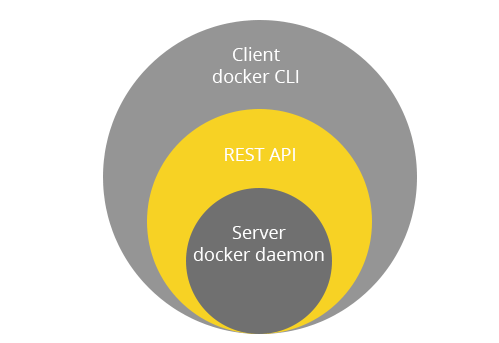
\includegraphics[width=0.7\textwidth]{wykorzystane_narzedzia/materialy/docker_structure.png}
 \label{fig:docker_structure}
\end{figure}\\
%
\textbf{Daemon Docker-a} jest centralnym miejscem, z kt�rego nast�puje zarz�dzanie kontenerami jak i obrazami. Dotyczy to zar�wno ich pobierania, budowy czy uruchamiania. Polecenia do wykonywania tych czynno�ci s� przesy�ane przez klienta z wykorzystaniem Docker REST API. Same obrazy s� natomiast przechowywane w repozytorium obraz�w, czy to publicznym czy prywatnym np. \textbf{Docker Hub}. W tym miejscu nale�y zaznaczy�, �e poza wieloma oficjalnymi obrazami udost�pniane s� r�wnie� nieoficjalne : budowane przez spo�eczno�� Docker-a.\\
%
W odr�nieniu od maszyn wirtualnych, kontenery wymagaj� du�o mniejszych zasob�w do samego uruchomienia, a i sam czas ich uruchomienia jest znacz�co ni�szy. Zosta�o to jednak uzyskane kosztem zmniejszenia izolacji pomi�dzy kontenerem, a samym systemem operacyjnym : poprzez wsp�dzielenie j�dra systemu.\\
%
\textbf{Obrazy} s� tak naprawd� szablonami w trybie read-only, z kt�rych kontenery s� uruchamiane. Sk�adaj� si� one z wielu warstw (layer-�w), kt�re, dzi�ki zastosowaniu ujednoliconego systemu plik�w (UFS), Docker ��czy w jeden konkretny obraz. Podstaw� ka�dego jest obraz bazowy, np. Ubuntu, na kt�ry nak�adane s� kolejne warstwy. Ka�da kolejna czynno�� (instrukcja) wykonywana na obrazie bazowym tworzy kolejn� warstw�, np. wykonanie komendy czy utworzenie pliku/katalogu. Komplet instrukcji tworz�cych obraz jest przechowywany w pliku Dockerfile. Podczas ��dania pobrania obrazu przez klienta, plik ten jest przetwarzany, czego wynikiem jest finalny obraz.\\
%
Poprzez zastosowanie warstw uzyskano bardzo niskie zu�ycie przestrzeni dyskowej, poniewa� podczas zmiany obrazu czy jego aktualizacji, budowana jest nowa warstwa, kt�ra zast�puje poprzedni� (aktualizowan�). Pozosta�e warstwy pozostaj� nienaruszone. Oznacza to, i� mo�liwe jest wsp�dzielenie warstw tylko do odczytu pomi�dzy kontenerami, czego efektem jest du�o ni�sze zu�ycie przestrzeni dyskowej, w por�wnaniu do standardowych VM.\\
%
\textbf{Registry}, czyli repozytorium obraz�w, jest faktycznym miejscem przechowywania obraz�w. Mo�e by� publiczne b�d� prywatne, lokalne b�d� zdalne. Najpopularniejszym repozytorium jest Docker Hub, kt�ry oferuje wiele dodatkowych funkcjonalno�ci, np. mo�liwo�� utworzenia repozytorium prywatnego. Oczywi�cie istniej� inne platformy, kt�re pozwalaj� na przechowywanie swoich obraz�w, jak np.  Quay.io, ale mo�liwe jest tak�e utworzenie w�asnej biblioteki : czy to lokalnie na komputerze, na kt�rym zosta� zainstalowany Docker czy zdalnie, na jednej z innych maszyn, kt�rymi zarz�dzamy.\\
%
Wspomniany wielokrotnie \textbf{kontener} to efekt ujednolicenia warstw tylko do odczytu oraz pojedynczej warstwy do odczytu i zapisu, dzi�ki kt�rej mo�liwe jest funkcjonowanie wymaganych zada�. Kontener wykonuje okre�lone wcze�niej zadanie, najcz�ciej jedno. Zawiera system operacyjny, pliki u�ytkownika, a tak�e tzw. metadane, dodawane automatycznie podczas tworzenia b�d� startu kontenera.\\
%
Kontener okre�lany jest r�wnie� jako �rodowisko wykonywalne Dockera. Mo�e przyjmowa� jeden z pi�ciu stan�w:
\begin{itemize}
\item created : utworzony, gotowy do uruchomienia,
\item up : dzia�aj�cy, wykonuj�cy zadanie,
\item exited : wy��czony, w trybie bezczynno�ci po zako�czeniu zadania,
\item paused : wstrzymany,
\item restarting : w trakcie ponownego uruchamiania.
\end{itemize}
%
Czas dzia�ania kontenera jest zale�ny od zadania, kt�re wykonuje. Samo uruchomienie sk�ada si� z siedmiu krok�w:
\begin{enumerate}
\item Pobrania wybranego obrazu, pod warunkiem, �e nie zosta� ju� pobrany wcze�niej.
\item Utworzenia kontenera.
\item Za�adowania systemu plik�w i utworzenia warstwy do odczytu i zapisu.
\item Zainicjowania sieci b�d� mostka sieciowego.
\item Konfiguracji sieci (adresu IP).
\item Uruchomienia zadania.
\item Przechwytywania wyj�cia i prowadzenia dziennika zdarze�.
\end{enumerate}
%
Mo�liwe jest ��czenie (linkowanie) kontener�w, przez co zyskuj� one bezpo�rednie po��czenie ze sob�. Same zadania wykonywane przez kontener s� tak samo wydajne, jakby by�y uruchamianie bezpo�rednio w systemie gospodarza.
 \section{Gazebo}
  
 \begin{figure}[htbp]
  \centering
  
\includegraphics[width=0.4\textwidth]{wykorzystane_narzedzia/materialy/gazebo.jpg}
  \label{fig:blender}
 \end{figure}
 
Symulator robot�w jest doskona�ym narz�dziem dla ka�dej osoby zajmuj�cej si� robotyk�. Pozwala szybko przetestowa� r�ne algorytmy i konstrukcje oraz skomplikowane systemy realizuj�ce niecodzienne scenariusze. Jednym z takich narz�dzi jest darmowy program Gazebo, przeznaczony do tworzenia dok�adnych i efektywnych symulacji 3D robot�w dzia�aj�cych w z�o�onych �rodowiskach. Posiada zaawansowany silnik fizyki, wysokiej jako�ci grafik� oraz wygodne i programowalne interfejsy. Symulator dost�pny jest dla systemu Linux na licencji Apache 2.0.
Program Gazebo powsta� na Uniwersytecie Po�udniowej Kalifornii jako cz�� systemu The Player Project, w kt�rego sk�ad wchodzi� r�wnie� symulator 2D - Stage. W 2011 roku symulator ten zosta� zintegrowany z bibliotekami Robot Operating System(ROS), co przyczyni�o si� do znacznego zwi�kszenia jego popularno�ci. Rozwojem Gazebo zajmuje si� teraz Open Source Robotic Foundation. Silnik graficzny wykorzystany w Gazebo to OGRE (Object Oriented Graphics Rendering Engine). Odpowiada on za wygl�d u�ytych modeli, o�wietlenie oraz cienie. Poprawnie odwzorowan� fizyk� (mi�dzy innymi model zderze� i kolizji) zapewnia silnik ODE (Open Dynamics Engine). Gazebo daje mo�liwo�� symulowania takich sensor�w jak: czujniki odleg�o�ci, kamery, skanery 3D czy modu�y GPS. Program pozwala na dodanie do ka�dego modelu kontrolera, steruj�cego jego prac�.Mo�liwe jest tworzenie prostych modeli bezpo�rednio w~Gazebo oraz importowanie bardziej z�o�onych, zaprojektowanych w zewn�trznych programach do grafiki 3D.
  
Podczas wyboru symulatora najistotniejsza by�a mo�liwo�� integracji z ROSem, a pod tym wzgl�dem Gazebo jest bezkonkurencyjne. Nie bez znaczenia jest r�wnie� dobra dokumentacja dost�pna na stronie http://gazebosim.org/.

% Krzysztof Kwieci�ski

\section{ROS}
%http://www.ros.org/about-ros/
%http://wiki.ros.org/ROS/Introduction
\textsf{ROS} jest meta-systemem operacyjnym rozwijanym w ramach ruchu wolnego oprogramowania. Zawiera: podstawowe procesy systemowe obs�uguj�ce urz�dzenia sprz�towe robota, sterowanie niskopoziomowe, implementacje wykonywania typowych funkcji, komunikacj� mi�dzyw�tkow� oraz zarz�dzanie pakietami. Opr�cz tego dostarcza u�ytkownikowi narz�dzia i~biblioteki pozwalaj�ce na tworzenie i~uruchomianie programu r�wnocze�nie na wielu komputerach. Jest platform� programistyczn� przeznaczon� do tworzenia oprogramowania steruj�cego robotami.
\textsf{ROS} jest szczeg�owo opisany na stronie internetowej projektu~\cite{website:gazebo}.  

\subsection{Struktura}
%http://rab.ict.pwr.wroc.pl/dydaktyka/instrukcje/ros_instrukcja.pdf
%http://wiki.ros.org/ROS/Concepts
Dzi�ki swojej strukturze (zbi�r narz�dzi, bibliotek i~konwencji) \textsf{ROS} znacz�co upraszcza proces modelowania z�o�onych zachowa� robota jednocze�nie zapewniaj�c �atwo�� przeno�no�ci kodu pomi�dzy r�nymi platformami robotycznymi. Zasada dzia�ania projektu w~\textsf{ROS} polega na komunikacji \textit{peer-to-peer} lu�no po��czonych ze sob� proces�w (mog� by� uruchomione na r�nych maszynach) za pomoc� infrastruktury komunikacyjnej zapewnianej przez platform�. Idea struktury �rodowiska przedstawiona jest na rysunku~\ref{fig:ros_struktura}.

%%http://rab.ict.pwr.wroc.pl/dydaktyka/instrukcje/ros_instrukcja.pdf
\begin{figure}[htbp]
 \begin{center}
  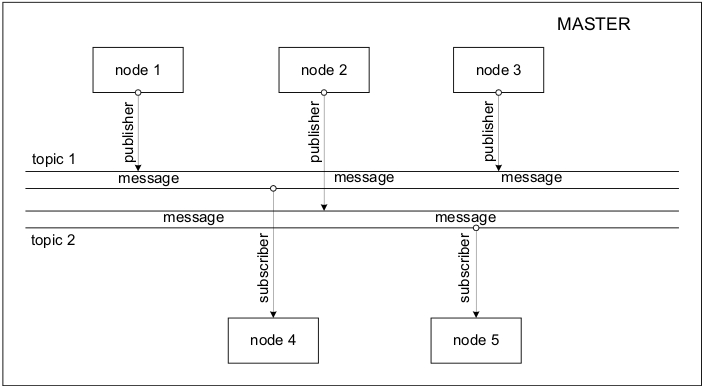
\includegraphics[width=\textwidth]{wykorzystane_narzedzia/materialy/ros_structure}    
  \caption{Schemat projektu na platformie \textsf{ROS} \cite{pwrinstrukcja}}
  \label{fig:ros_struktura}
 \end{center}
\end{figure} 

\subsubsection{Pakiety (\textit{packages})}
%http://wiki.ros.org/ROS/Concepts
Pakiety s� g��wn� jednostk� s�u��c� do organizacji oprogramowania. Mog� zawiera�: w�z�y, biblioteki zale�ne od \textsf{ROS}a, zbiory danych, pliki konfiguracyjne lub inne elementy u�ytecznie powi�zane ze sob�. Pakiety s� najmniejsz� jednostk� budulcow� systemu \textsf{ROS}, czyli najmniejsz� rzecz�, kt�r� mo�na zbudowa� i~udost�pni�. Ka�dy z~nich zawiera dokumentacj� (\textit{manifest}) opisan� w~pliku \texttt{package.xml}.

\subsubsection{W�z�y (\textit{nodes})}
%http://wiki.ros.org/ROS/Concepts
W�z�y s� wykonywalnymi instancjami program�w �rodowiska \textsf{ROS}.
System sterowania robotem zazwyczaj sk�ada si� z~wielu w�z��w. Przyk�adowo dla jednego robota mobilnego mo�na wyr�ni� kilka w�z��w odpowiadaj�cych za r�ne funkcjonalno�ci: skaner laserowy, silniki, lokalizacj�, planowanie ruchu itd.
Wyr�nia si� r�wnie� w�ze� nadrz�dny \texttt{master}, kt�ry odpowiada za poprawno�� komunikacji mi�dzy wszystkimi w�z�ami systemu.

\subsubsection{Tematy (\textit{topics}) i wiadomo�ci (\textit{messages})}
%http://wiki.ros.org/ROS/Concepts
W�z�y porozumiewaj� si� ze sob� poprzez przesy�anie wiadomo�ci. Wiadomo�� jest prost� struktur� danych, w~kt�rej znajdowa� si� mog� pola r�nych typ�w prostych oraz tablic typ�w prostych. Co istotne, struktura mo�e mie� zagnie�d�on� budow�, czyli sk�ada� si� z~dowolnej liczby zagnie�d�onych struktur i~tablic. Wiadomo�ci s� przesy�ane poprzez system transportowy zorganizowany na zasadzie nadawca--odbiorca (\textit{publisher}-- \textit{subscriber}).

W�ze� wysy�a wiadomo�� poprzez opublikowanie jej w danym temacie. Temat jest nazw� s�u��c� do identyfikacji zawarto�ci wiadomo�ci. W�ze� odbieraj�cy �ledzi wybrane tematy i~otrzymuje wiadomo�ci wysy�ane do nich. Mo�e by� wiele r�wnoczesnych nadawc�w i~odbiorc�w dla jednego tematu oraz jeden w�ze� mo�e publikowa� i~subskrybowa� wiele temat�w. Poszczeg�lne w�z�y uczestnicz�ce w~komunikacji nie s� �wiadome istnienia innych. Odpowiada to idei roz��czenia produkcji danych od ich konsumpcji.

\subsubsection{Us�ugi (\textit{services})}
%http://wiki.ros.org/ROS/Concepts
Us�ugi udost�pniaj� inny mechanizm komunikacji pomi�dzy w�z�ami. Us�uga jest zdefiniowana poprzez par� struktur wiadomo�ci: jedn� dla ��dania, drug� dla odpowiedzi. W~przeciwie�stwie do prostego przesy�ania wiadomo�ci, kt�re przekazywane s� w~jednym kierunku na zasadzie wiele-do-wielu, us�ugi pozwalaj� na interakcj� ��danie/odpowied�. Takie podej�cie jest cz�sto wymagane w rozproszonym systemie. W�ze�-serwer oferuje us�ug� o danej nazwie, natomiast w�ze�-klient korzysta z~niej poprzez zg�oszenie wiadomo�ci ��dania, a~nast�pnie oczekiwanie na odpowied�. 

\subsubsection{Worki (\textit{bags})}
%http://wiki.ros.org/ROS/Concepts
Worki s� formatem zapisu i~odtwarzania informacji zawartych w wiadomo�ciach. Jest to istotny mechanizm s�u��cy do przechowywania danych, kt�re mog� by� trudne do zebrania np. danych sensorycznych. Umo�liwiaj� r�wnie� testowanie program�w dla jednolitego, uprzednio zdefiniowanego, zestawu danych.
\newpage
\section{Qt}
\begin{figure}[htbp]
 \centering
 
\includegraphics[width=0.4\textwidth]{wykorzystane_narzedzia/materialy/QT.png}
 \label{fig:QTlogo}
\end{figure}
Qt jest to wieloplatformowy zestaw narz�dzi i bibliotek dedykowany dla j�zyka C++. �rodowisko to jest dost�pne dla takich platform jak X11 (m. in. GNU/LINUX, BSD, Solaris), Windows, Mac OS X oraz dla urz�dze� wbudowanych opartych na lineksie, Windows CE, Symbian czy Android. 
Podstaw� dzia�ania bibliotek Qt jest mechanizm slot�w i sygna��w, kt�re zapewniaj� obs�ug� wszelkich zdarze� w obr�bie aplikacji i s�u�y komunikacji pomi�dzy objektami. Odbywa si� to w spos�b nast�puj�cy, podczas dzia�ania naszej aplikacji pewne specyficzne akcje, predefiniowane b�d� dodane przez u�ytkownika, emituj� sygna� zawieraj�cy informacje o danym zdarzeniu. Slot natomiast jest to funkcja, kt�ra zostaje wywo�ana jako reakcja na wze�niej przypisany jej konkretny sygna�. 
\newline
Wa�nym przy wyborze narz�dzi do zaimplementowania prostego GUI na potrzeby realizowanego projektu by� fakt, i� ca�y interfejs symulatora Gazebo zosta� oparty w�a�nie o omawiane tutaj biblioteki. Dodatkowo posiada on do�� du�e wsparcie dla tworzenia w�asnych plugin�w zintegrowanych z owym �rodowiskiem, co znacz�co wp�yn�o na komfort korzystania z naszej aplikacji. Nale�y r�wnie� wspomnie� o prostocie wykorzystywania tego rozwi�zania. Znacz�c� cz�� pracy wykonuje MOC (Qt Meta Object Compiler), generuj�c kod odpowiedzialny za obs�ug� wszystkich mechanizm�w bibliotek Qt, z kt�rych w danej aplikacji korzystamy. Dzi�ki temu tw�rcy tego rozwi�zania w bardzo du�ym stopniu upro�cili oraz przyspieszyli procedur� pisania kodu przez programist�. 
Pos�uguj�c si� owymi bibliotekami w wersji Qt4 i ich podstawowymi klasami stworzono kilka prostych okien, w kt�rych mie�ci si� niemal�e ca�o�� funkcjonalno�ci naszego projektu. W ten spos�b stworzona zosta�a belka z przyciskami zakotwiczona w interfejsie symulatora a tak�e wsomniane wcze�niej okna daj�ce u�ytkownikowi mo�liwo�� kontrolowania symulacji czy zarz�dzania naszymi modelami robot�w b�d� sali. Owe okna oraz dostarczona przez nie funkcjonalno�� jest szczeg�owo opisana w dalszej cz�ci raportu.
\section{Inventor}
\section{Blender}

\begin{figure}[htbp]
 \centering
 
\includegraphics[width=0.4\textwidth]{wykorzystane_narzedzia/materialy/blender.jpg}
 \label{fig:blender}
\end{figure}

Blender jest bezp�atnym narz�dziem do tworzenia grafiki 3D. Umo�liwia projektowanie oraz renderowanie zar�wno statycznych modeli, jak i animacji, czy gier.

Oprogramowanie to posiada pot�ne mo�liwo�ci, dzi�ki czemu z powodzeniem mo�e konkurowa� z profesjonalnymi, p�atnymi programami takimi jak 3DS Max, czy Maya. Dzi�ki du�ej popularno�ci i ogromnej rzeszy u�ytkownik�w posiada wsparcie spo�eczno�ci. W po��czeniu z licencj� open-source i mo�liwo�ci� edycji kodu daje on niemal nieograniczone mo�liwo�ci przy tworzeniu wszelkiego rodzaju plugin�w. Dzi�ki mo�liwo�ci u�ywania skrypt�w w Pythonie jego funkcjonalno�� mo�na rozszerza� i automatyzowa�.

W przeciwie�stwie do Inventora, modele od pocz�tku i w ca�o�ci s� projektowane w widoku 3D. Wynika to z faktu, i� Blender znajduje zastosowania g��wnie przy tworzeniu grafiki wirtualnej, a nie przy projektach technicznych. W takim przypadku tego typu podej�cie do projektowania lepiej si� sprawdza.
Blender umo�liwia eksport do formatu Collada (.dae). Funkcja ta by�a kluczowa z powodu konieczno�ci wykorzystania tego w�a�nie formatu przy tworzeniu modeli do symulacji w Gazebo.

\section{Zarz�dzanie projektem}
\subsection{Git}
\subsection{Trello}

\chapter{Opis systemu}

Symulator robot�w jest doskona�ym narz�dziem dla ka�dej osoby zajmuj�cej si� robotyk�. Pozwala szybko przetestowa� r�ne algorytmy i konstrukcje oraz skomplikowane systemy realizuj�ce niecodzienne scenariusze. Jednym z takich narz�dzi jest darmowy program Gazebo, przeznaczony do tworzenia dok�adnych i efektywnych symulacji robot�w dzia�aj�cych w z�o�onych �rodowiskach. Posiada zaawansowany silnik fizyki, wysokiej jako�ci grafik� oraz wygodne i programowalne interfejsy.
\\ \\
To powy�ej to pr�ba t�umaczenia opisu poni�ej ze strony Gazebo :D
\\ \\
Robot simulation is an essential tool in every roboticist's toolbox. A well-designed simulator makes it possible to rapidly test algorithms, design robots, perform regression testing, and train AI system using realistic scenarios. Gazebo offers the ability to accurately and efficiently simulate populations of robots in complex indoor and outdoor environments. At your fingertips is a robust physics engine, high-quality graphics, and convenient programmatic and graphical interfaces. Best of all, Gazebo is free with a vibrant community.

\section{Okienka}
Funkcjonalno�ci + Implementacja
\subsection{Konfiguracja �wiata}
\begin{figure}[htbp]
 \centering
 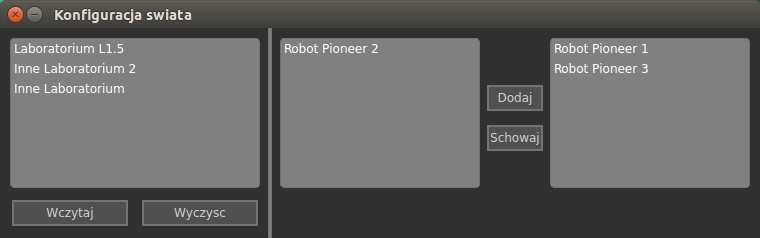
\includegraphics[width=1.0\textwidth]{opis_systemu/materialy/konfiguracja_swiata.jpeg}
 \label{fig:konfiguracja_swiata}
 \caption{Okno konfiguracji �wiata}
\end{figure}

Okno konfiguracji �wiata pozwala zmodyfikowa� zawarto�� sceny. Domy�lnie �adowany jest jedynie ground plane, czyli bazowe pod�o�e, na kt�rym umieszczane s� modele. Okno umo�liwia szybkie rozpocz�cie pracy z wybranymi modelami. U�ytkownik ma mo�liwo�� wyboru sali z listy dost�pnej w lewej cz�ci okna. Lista tworzona jest na podstawie plik�w konfiguracji sali z rozszerzeniem .txt znajduj�cych si� w folderze worlds, w katalogu �r�d�owym Gazebo. Przyk�adowy zestaw danych ma nast�puj�c� posta�:
\begin{lstlisting}[language=bash]
smietnik 4.6 1.3 0 0 0 0
szafa 1.5 -3.6 0 0 0 0
kaloryfer -4.5 1.6 0 0 0 1.570796
kaloryfer -4.5 -2.8 0 0 0 1.570796
stol -2.4 2.5 0 0 0 0
stol -4 2.5 0 0 0 0
stol -0.7 -3.4 0 0 0 0
krzeslo -1.7 -2.6 0 0 0 0
krzeslo -1 -2.6 0 0 0 0
krzeslo -0.1 -2.6 0 0 0 0
\end{lstlisting}
W ka�dej linii dodawany jest jeden z dost�pnych modeli. Trzy pierwsze liczby oznaczaj� pozycj� modelu na scenie (X, Y, Z). Pozosta�e okre�laj� orientacj� wok� ka�dej z osi.

Naci�niecie przycisku "Wczytaj" powoduje wyczyszczenie sceny i za�adowanie wybranej sali. Przycisk "Wyczy��" usuwa wszystkie statyczne modele.

Prawa strona okna konfiguracji �wiata pozwala wybra� liczb� robot�w Pioneer, z kt�rymi u�ytkownik chce rozpocz�� prac�. Liczba pozycji w lewym polu okre�la ile robot�w jest dost�pnych, natomiast liczba pozycji w prawym polu definiuje liczb� robot�w na scenie. Zawarto�� p�l mo�na modyfikowa� za pomoc� przycisk�w "Dodaj" i "Schowaj".
% Krzysztof Kwieci�ski
\subsection{Zarz�dzanie robotami}
Okienko \texttt{Zarz�dzanie robotami} umo�liwia ustawianie pozycji oraz orientacji wybranego robota na scenie.

Zak�adki umo�liwiaj� wyb�r \texttt{Pioneera}, kt�rego pozycj� chcemy zmieni�. Aktywne s� tylko zak�adki skojarzone z~robotami dodanymi aktualnie do �wiata. 

Po wyborze zak�adki mo�liwe jest podanie nowych wsp�rz�dnych $XY$ oraz orientacji $\theta$ robota. W~polach odpowiedzialnych za pozycj� i~orientacj� kolor informuje o~poprawno�ci wprowadzonych danych -- zielony oznacza poprawnie wype�nione pola, natomiast czerwony b��dnie. 

Przyci�ni�cie przycisku \texttt{Ustaw} powoduje ustawienie \texttt{Pioneera} zgodnie z~��daniem. Przycisk \texttt{Reset} przenosi robota do punktu $(0, 0)$ i~ustawia jego orientacj� na~$0$. 

Po zmianie zak�adki lub ustawieniu/zresetowaniu pozycji, w~polach wy�wietlane s� aktualne wsp�rz�dne robota.

\begin{figure}[htbp]
 \centering
 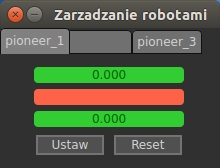
\includegraphics[]{opis_systemu/materialy/zarzadzanie_robotami.jpeg}
 \label{fig:zarzadzanie_robotami}
 \caption{Okno zarz�dzania robotami}
\end{figure}

\subsubsection{Implementacja}
Klasa odpowiadaj�ca za ca�e okienko to \texttt{RobotManagementWindow}. Dziedziczy ona po klasie \texttt{QDialog}. 

Sloty odpowiadaj�ce za to co dzieje si� w~oknie w~momencie dodania lub schowania robota to:
\begin{lstlisting}[language=C++, numbers=none]
public slots:
	void onAddRobot(int id);
	void onHideRobot(int id);
\end{lstlisting}
W~momencie otrzymania odpowiednich sygna��w aktywowana b�d� dezaktywowana jest stosowna zak�adka, a~tak�e ustawiane s� warto�ci w~polach.

Wy�wietlanie pozycji i~orientacji robota mo�liwe jest dzi�ki subskrybowaniu odpowiedniego tematu i~wywo�aniu funkcji aktualizuj�cej pozycj� robota:
\begin{lstlisting}[language=C++, numbers=none]
this->sub = node->Subscribe("~/pose/info", 
                            &RobotManagementWindow::OnPoseMsg, this);
\end{lstlisting}

Klasa odpowiadaj�ca za wygl�d  pojedynczej zak�adki oraz g��wn� funkcjonalno�� okienka to \texttt{RobotManagementTab}. Dziedziczy ona po klasie \texttt{QWidget}. Jej kluczowe metody to:
\begin{lstlisting}[language=C++, numbers=none]
private slots:
	void on_pushButtonUstaw_clicked();
	void on_pushButtonReset_clicked();
\end{lstlisting}
Odpowiadaj� one za ustawienie b�d� zresetowanie pozycji robota. Przyci�ni�cie kt�rego� z~przycisk�w skutkuje wywo�aniem us�ugi \texttt{/gazebo/set\_model\_state}.














\subsection{Wyniki symulacji}

\input{opis_systemu/wyniki_symulacji/funkcjonalnosc}
\input{opis_systemu/wyniki_symulacji/implementacja}
\section{Pluginy}
Plugin, czyli wtyczka, jest cz�ci� kodu, kt�ry zosta� skompilowany jako wsp�dzielona biblioteka i dodany do symulatora. Ma on dost�p do wszystkich funkcjonalno�ci Gazebo poprzez gotowe klasy j�zyka C++. Pluginy s� bardzo przydatne nie tylko ze wzgl�du na mo�liwo�� kontroli dowolnych modu��w symulatora, ale r�wnie� ze wzgl�du na swoj� elastyczno��. Z �atwo�ci� mo�na je dodawa� i usuwa� z systemu. W Gazebo jest dost�pnych 6 typ�w wtyczek:
\begin{itemize}
\item World
\item Model
\item Sensor
\item System
\item Visual
\item GUI
\end{itemize}
Oprogramowanie utworzone w ramach projektu wykorzystuje dwie z nich: GUI i World.
\subsection{GUI}
Plugin GUI jest bezpo�rednio zwi�zany z graficznym interfejsem u�ytkownika. Z jego poziomu mo�na w prosty spos�b dodawa� elementy takie jak przyciski, okna, listy czy pola tekstowe. Wtyczka dodawana jest do pliku konfiguracji �wiata w nast�puj�cy spos�b:
\begin{lstlisting}[language=bash]
...
<gui fullscreen='0'>
<plugin name='SimulationGUI' filename='lib_simulation_gui_plugin.so'/>
...
\end{lstlisting}
Z wykorzystaniem pluginu GUI i bibliotek Qt utworzona zosta�a w g�rnej cz�ci okna symulacji belka z trzema przyciskami otwieraj�cymi opisane wcze�niej okna konfiguracyjne, zwi�kszaj�ce funkcjonalno�� symulatora.

Wtyczka interfejsu ma ograniczony dost�p do zasob�w Gazebo. Chc�c z jej pomoc� dokonywa� modyfikacji na scenie konieczne jest wysy�anie odpowiednich komend do pluginu World. W tym celu w projekcie wykorzystano komunikacj� za pomoc� temat�w symulatora. Wtyczka GUI pe�ni rol� nadawcy (publisher), natomiast wtyczka World jest subskrybentem (subscriber). Wiadomo�ci mog� mie� dowolny, wcze�niej zdefiniowany format. Przyk�adowo, je�eli wysy�ane s� informacje o pozycji robota, format wiadomo�ci zawiera nazw� modelu i sze�� zmiennych liczbowych przechowuj�cych pozycj� i orientacj�.

Tworzenie temat�w i konfiguracja komunikacji realizowana jest z poziomu kodu, z~wykorzystaniem bibliotek Gazebo.

\subsection{World}
World plugin pozwala na edycj� r�nych parametr�w �wiata, przyk�adowo silnika fizyki lub o�wietlenia. Ponadto umo�liwia modyfikowanie sceny i znajduj�cych si� na niej obiekt�w. Wtyczka jest bezpo�rednio zwi�zana z plikiem ustawie� z rozszerzeniem .world, �adowanym podczas uruchamiania Gazebo. Ten plik jest r�wnie� odpowiedzialny za uruchomienie wybranej wtyczki:
\begin{lstlisting}[language=bash]
<sdf version='1.6'>
<world name='default'>
<plugin name='projekt_przejsciowy' filename='libprojekt_przejsciowy.so'/>
...
\end{lstlisting}
Budowa pluginu World w pliku �r�d�owym jest do�� prosta i intuicyjna. Minimalny kod pozwalaj�cy skompilowa� bibliotek� ma nast�puj�c� posta�:
\begin{lstlisting}[language=bash]
#include <gazebo/gazebo.hh>

namespace gazebo
{
  class WorldPluginTutorial : public WorldPlugin
  {
    public: WorldPluginTutorial() : WorldPlugin()
    {
      printf("Witaj!\n");
    }
    public: void Load(physics::WorldPtr _world, sdf::ElementPtr _sdf)
    {
    }
  };
  GZ_REGISTER_WORLD_PLUGIN(WorldPluginTutorial)
}
\end{lstlisting}
Na podstawie powy�szego kodu, przy odpowiedniej konfiguracji plik�w makefile mo�na zbudowa� plik z rozszerzeniem .so, kt�ry jako biblioteka jest dodawany do programu.
\section{Integracja Gazebo z ROS}
G��boka integracja Gazebo z ROS jest najwi�ksz� zalet� tego symulatora. Umo�liwia j� zestaw dostarczanych plugin�w do ROS w pakiecie gazebo\_ros\_pkgs.
Podstawowe funkcjonalno�ci dostarczane razem z pakietem:
\begin{itemize}
\item pomimo integracji Gazebo pozostaje nadal samodzielnym systemem,
\item mo�liwo�� zbudowania pakiet�w Gazebo w catkin,
\item zmniejszenie ilo�ci kodu potrzebnego do symulacji,
\item udost�pnia u�ytkownikowi szereg us�ug i temat�w ROS do zarz�dzania symulacj� (wymienione na Rysunku \ref{fig:ros_integracja})
\end{itemize}

\begin{figure}[htbp]
 \begin{center}
  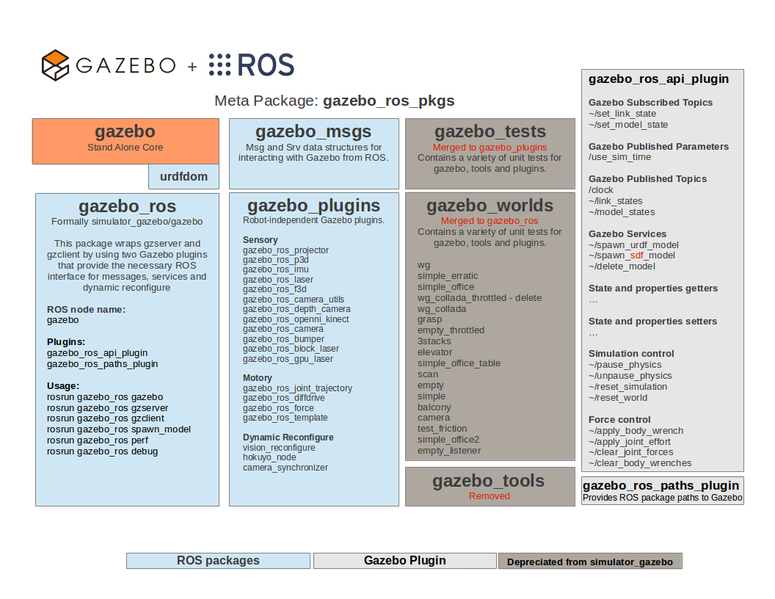
\includegraphics[width=\textwidth]{opis_systemu/materialy/gazeborosapi}   
  \caption{Schemat prezentuj�cy funkcje udost�pniane przez gazebo\_ros\_pkgs}
  \label{fig:ros_integracja}
 \end{center}
\end{figure} 

\subsection{Kompilacja pakiet�w Gazebo przy u�yciu catkin}
Jak zaznaczono wcze�niej, mo�liwe jest bezpo�rednie u�ycie systemu catkin do budowania pakiet�w napisanych dla Gazebo. Wymaga�o to stworzenia catkin workspace -- katalogu, w kt�rym budowane s� pakiety catkin. Stworzone przez nas pluginy Gazebo zosta�y zebrane i tak skonfigurowane, �e tworz� pakiet kompatybilny z ROS.

Po uruchomieniu, Gazebo tworzy w�asny w�ze� do komunikacji z ROS. Dzi�ki kompilacji poprzez catkin, pluginy Gazebo maj� dost�p do ROSa, bezpo�rednio w kodzie mo�emy odwo�ywa� do jego funkcji. Aby si� o tym upewni�, w World plugin umieszczono poni�szy kod, kt�ry zatrzymuje dzia�anie Gazebo w przypadku braku komunikacji z ROS.

\begin{lstlisting}[language=c]
...                                                                                   
if ( !ros::isInitialized() )
{
	ROS_FATAL_STREAM("A ROS node for Gazebo has not been initialized");
	return;
}
...
\end{lstlisting}

\subsection{Uruchamianie Gazebo przy u�yciu narz�dzi z ROS}
Dzi�ki u�yciu catkin'a mo�emy uruchamia� Gazebo za pomoc� narz�dzia roslaunch, kt�re pozwala na automatyczne wywo�ywanie w�z��w ROS oraz wst�pn� konfiguracj�. U�atwia to start skonfigurowanego do pracy �rodowiska, co sprowadza si� do jednego polecenia:
\begin{verbatim}
$ roslaunch projekt_przejsciowy l15.launch
\end{verbatim}
Aby to umo�liwi�, przygotowano odpowiedni plik l15.launch w podkatalogu stworzonego pakietu Gazebo $launch$. Plik launch mo�e przy uruchomieniu wczytywa� plik world z~konfiguracj� Gazebo lub umieszcza� modele w odpowiednich miejscach.

\subsection{Udost�pnione funkcjonalno�ci do komunikacji ROS}
Jak wida� na Rysunku \ref{fig:ros_integracja}, Gazebo udost�pnia szereg funkcjonalno�ci kt�rych mo�na u�y� do integracji z ROS. 

Dla projektu najwi�ksze znaczenie mia�y pluginy wysy�aj�ce dane z czujnik�w na robocie, takich jak skaner laserowy czy kamera oraz umo�liwiaj�ce sterowanie nap�dem robota. Zosta�y one zintegrowane z modelem Pioneera.

W�ze� tworzony przez Gazebo publikuje informacje na zewn�trz za pomoc� temat�w, np. \~/model\_states, wysy�aj�cy informacje o stanie modeli aktualnie u�ywanych w symulacji. W�ze� dostarcza r�wnie� us�ugi ROS'a, takie jak \~/spawn\_urdf\_model do �adowania modeli robot�w w formacie URDF, czy \~/delete\_model do usuwania modeli. Mog� zosta� one wykorzystane przez u�ytkownika naszego systemu do kontroli symulacji i zbierania danych symulacyjnych.
\section{Modele}

Modele u�yte do stworzenia laboratorium L1.5 zosta�y wykonane w programach Inventor Professional oraz Blender.

Elementy wyposa�enia wn�trza takie jak sto�y, krzes�a, grzejniki, szafa oraz �mietnik zaprojektowane zosta�y w Inventorze, natomiast sama sala (�ciany) w programie Blender. Wszystkie stworzone elementy opracowane zosta�y w oparciu o pomiary rzeczywistych mebli, przedmiot�w i �cian w sali L1.5 w budynku C-16. Nast�pnie wszystkie elementy zosta�y przekonwertowane przy u�yciu programu Blender do formatu Collada (.dae), aby mo�liwe by�o wykorzystanie ich w Gazebo.

Modele zosta�y r�wnie� posk�adane w Blenderze w celu wyrenderowania widok�w z r�nych miejsc sali:

\begin{center}

	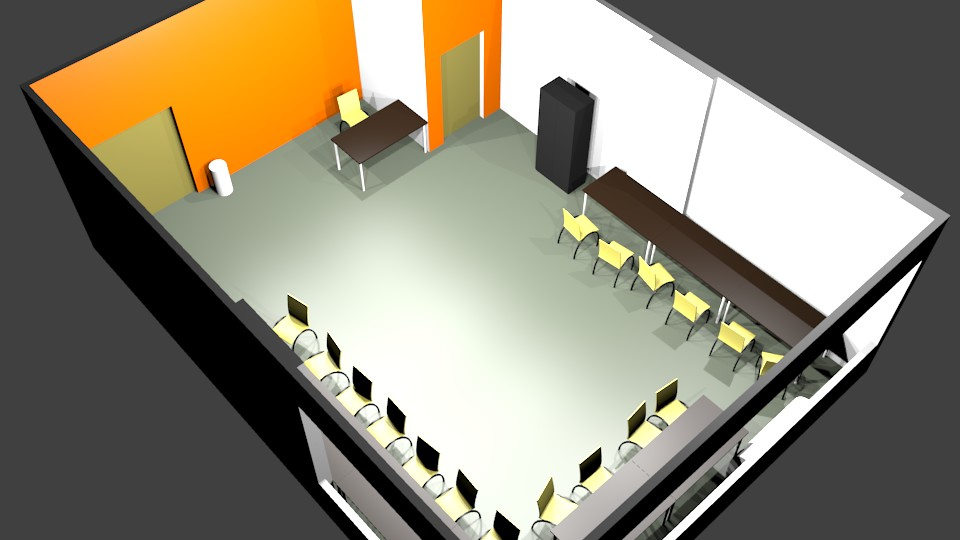
\includegraphics[width=12cm]{opis_systemu/materialy/R4.jpg}
	
	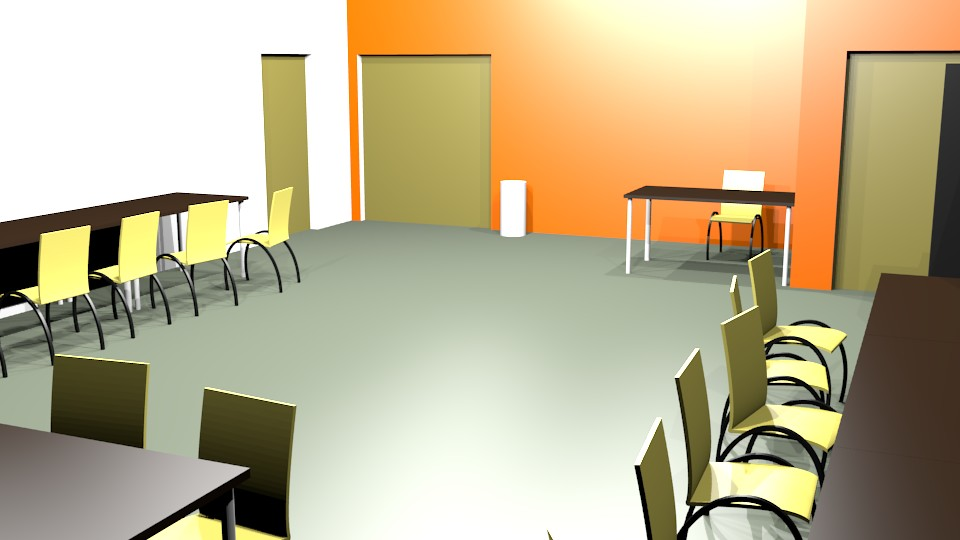
\includegraphics[width=12cm]{opis_systemu/materialy/R1.jpg}

\end{center}

Aby stworzone modele mog�y by� u�yte w Gazebo, konieczne by�o jeszcze napisanie plik�w konfiguracyjnych "model.config" oraz "model.sdf".
\\
Plik "model.config" zawiera takie informacje jak:
\begin{itemize}
\item nazwa obiektu
\item lista wersji pliku .sdf
\item informacje o autorze
\end{itemize}
W pliku "model.sdf" przechowywane s� informacje na temat:
\begin{itemize}
\item w�a�ciwo�ci fizycznych obiektu (masa, momenty bezw�adno�ci)
\item statyczno�ci obiektu (mo�liwo�ci poruszenia przez inny obiekt)
\item geometrii obiektu wyko�ystywanej przy kolizji z innymi obiektami
\item wizualizacji obiektu w symulacji
\end{itemize}
W przypadku modeli z�o�onych, takich jak np. roboty, plik "model.sdf" mo�e zawiera� r�wnie�:
\begin{itemize}
\item informacje o w�a�ciwo�ciach fizycznych poszczeg�lnych cz�on�w obiektu
\item parametry po��cze� kinematycznych mi�dzy cz�onami
\item pluginy wyko�ystywane w modelu
\item dane o czujnikach i ich umieszczeniu
\end{itemize}
Do stworzenia modelu robota Pioneer wykorzystano pliki zawarte w Gazebo, jednak aby mo�na by�o go u�y� w symulacjach konieczne by�o zaimplementowanie jego funkcjonalno�ci w pliku .sdf. W tym celu dodano pluginy do obs�ugi nap�d�w oraz sensor�w, kt�re zosta�y dodane do modelu.

Dzi�ki tym zabiegom podczas dodawania robota w symulacji tworzone s� tematy pozwalaj�ce na komunikacj� z modelem robota.
\chapter{Testy}

W ramach test�w systemu przygotowano �rodowisko zgodnie z instrukcj� u�ytkownika (zawarta w dodatku A). Po uruchomieniu systemu symulacyjnego wykonano czynno�ci sprawdzaj�ce dzia�anie podstawowych funkcji oprogramowania, wymaganych do bezproblemowego u�ytkowania go.

W pierwszej kolejno�ci sprawdzono poprawno�� wczytywania si� modelu laboratorium, oraz umieszczania i chowania robot�w ze sceny, test ten wypad� pomy�lnie.
Kolejnym wa�nym aspektem jest to czy w systemie ROS, po dodaniu robota pojawiaj� si� odpowiednie tematy. Dla robota 'pioneer\_1' s� to:

\begin{itemize}
\item \begin{verbatim}/pioneer_1/RosAria/cmd_vel\end{verbatim}
\item \begin{verbatim}/pioneer_1/RosAria/pose \end{verbatim}
\item \begin{verbatim}/pioneer_1/camera/camera_info\end{verbatim}
\item \begin{verbatim}/pioneer_1/camera/image_raw\end{verbatim}
\item \begin{verbatim}/pioneer_1/camera/parameter_descriptions\end{verbatim}
\item \begin{verbatim}/pioneer_1/camera/parameter_updates\end{verbatim}
\item \begin{verbatim}/pioneer_1/scan\end{verbatim}
\end{itemize}


\begin{figure}[htbp]
 \centering
 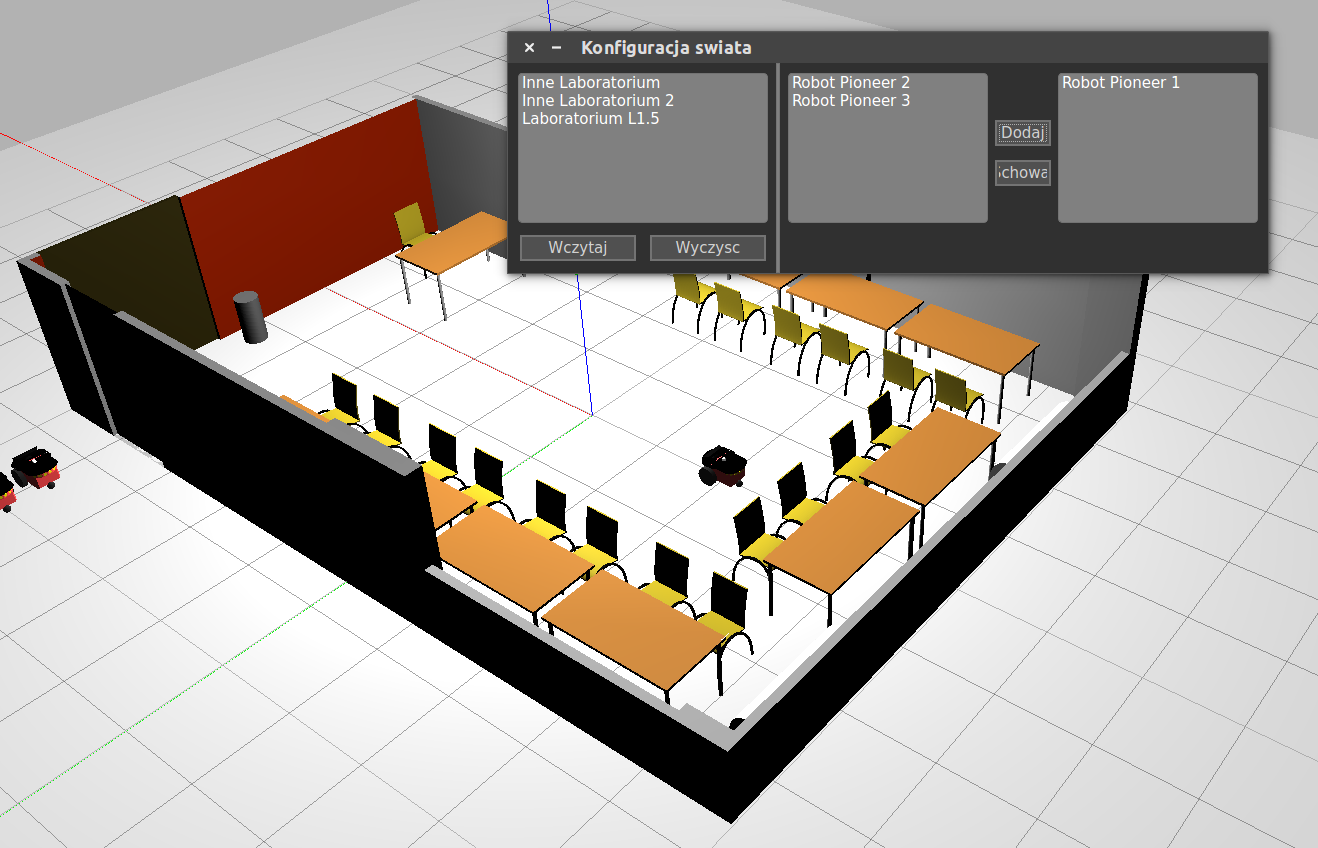
\includegraphics[width=0.8\textwidth]{testy/test1.png}
 \label{fig:docker}
\end{figure}


Nast�pnie sprawdzono mo�liwo�� zarz�dzania pozycj� robot�w z poziomu okienka \texttt{Zarz�dzanie robotami}. Przeprowadzone testy wykaza�y, �e pozycja robota ustawiana jest w~spos�b odpowiedni, a b��dnie wprowadzone dane s� odpowiednio sygnalizowane. Jedynym problemem okaza� si� brak weryfikacji czy miejsce w kt�rym chcemy postawi� robota jest wolne i czy nie wyl�duje on np. na innym robocie.


Ostatni� grup� funkcjonalno�ci jest mo�liwo�� rejestracji pozycji robota i zapisanie jej do pliku. W celu weryfikacji do systemu ROS opublikowano dwie wiadomo�ci, kt�re w~efekcie powinny umo�liwi� narysowanie robotem �semki:
\begin{itemize}
\item \begin{verbatim}rostopic pub /pioneer_1/RosAria/cmd_vel \
geometry_msgs/Twist -- '[0.5, 0.0, 0.0]' '[0.0, 0.0, 0.2]' \end{verbatim}
\item \begin{verbatim}rostopic pub /pioneer_1/RosAria/cmd_vel \
geometry_msgs/Twist -- '[0.5, 0.0, 0.0]' '[0.0, 0.0, -0.3]' \end{verbatim}
\end{itemize}

Po wykonaniu powy�szych polece� robot pokona� zamierzon� tras�, a otrzymane wykresy ruchu zgadza�y si� z oczekiwaniami.

\begin{figure}[htbp]
 \centering
 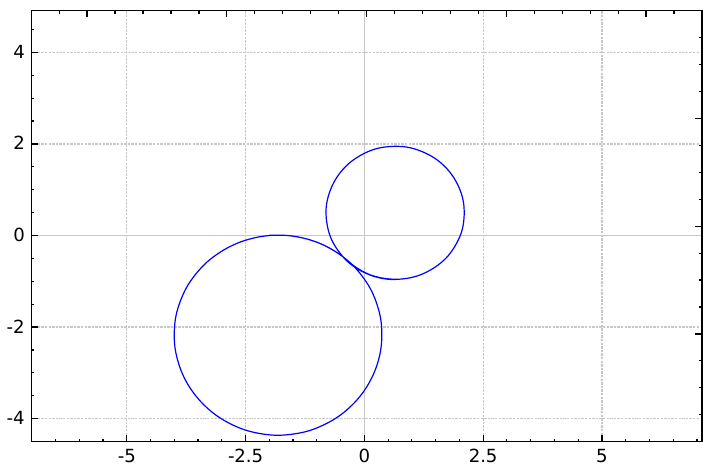
\includegraphics[width=0.6\textwidth]{testy/test3.png}
 \label{fig:docker}
\end{figure}


\section{Przygotowanie do laboratorium}

W celu sprawdzenia mo�liwo�ci korzystania z modu�u RosAriaDriver, napisano prosty program umo�liwiaj�cy poruszanie si� po kwadracie, z wykorzystaniem napisanej w~j�zyku Python biblioteki drive\_simulation.py dost�pnej w przygotowanym kontenerze Dockera.
\begin{verbatim}
from drive_simulation import RosAriaDriver
p = RosAriaDriver('pioneer_1')
for i in range(4):
    p.SetSpeedLR(0.2, 0.2, 5)
    p.SetSpeed(0, 0.2, 5)
\end{verbatim}

W ten spos�b uda�o si� uzyska� przejazd po �cie�ce przypominaj�cej kwadrat.

\begin{figure}[htbp]
 \centering
 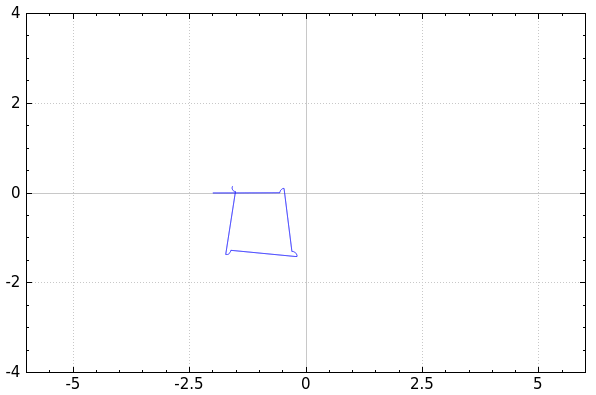
\includegraphics[width=0.6\textwidth]{testy/test4.png}
 \label{fig:docker}
\end{figure}

\chapter{Podsumowanie i wnioski}
Realizacja tego projektu mia�a dwa g��wne cele. Pierwszym z nich by�o opracowanie systemu pozwalaj�cego na wst�pne przeprowadzenie �wicze� laboratoryjnych jeszcze przed przyst�pieniem do zaj��. Drugim aspektem zadania by�o pokazanie studentom uczestnicz�cym w kursie Projekt przej�ciowy jak w praktyce wygl�da praca nad produktem w stosunkowo du�ych grupach projektowych oraz nauczenie ich korzystania z~narz�dzi do zarz�dzania prac�, planowania zada�, kontrolowania poczynionych post�p�w czy zapewniaj�cych komunikacj� wewn�trz grupy. 

\section{Serwer}

\section{Zastosowanie kontener�w}
Branymi pod uwag� opcjami udost�pnienia tworzonej aplikacji i jej sk�adowych by�o spakowanie ca�o�ci do obrazu maszyny wirtualnej b�d� kontenera. Jako l�ejsz� i bardziej przyst�pn� wybrali�my drug� opcj�. Pozwoli�o to w znacz�cy spos�b ograniczy� wielko�� wynikowej paczki a dzi�ki bardzo szybkiemu rozwojowi tej technologii w ostatnich latach cieszy si� ona ogromnym zainteresowaniem i dobrym wsparciem technicznym. Bogata dokumentacja i zasoby tutoriali pozwoli�y na szybkie wdro�enie owych mechanizm�w do naszego projektu. Dodatkowo, bardzo pomocne by�o internetowe repozytorium s�u��ce do przechowywania takich kontener�w, dzi�ki czemu ka�da modyfikacja sprowadza�a si� do zaktualizowania obrazu na serwerze i pobrania go przez wszystkich pracuj�cych z danym kontenerem nowych plik�w i zasob�w zamiast ka�dorazowego pobierania ca�ej paczki z zewn�trznego, cz�sto wolniejszego serwera. Takie rozwi�zanie poci�ga za sob� wielk� wygod� dla os�b korzystaj�cych z naszego projektu -- udost�pniona przez nas paczka zawiera kompletne �rodowisko, zainstalowane wszystkie niezb�dne pakiety i aplikacje, kt�re, pr�buj�c uruchomi� nasze dzie�o na czystym systemie, nale�a�oby pobra� i zainstalowa�. Ca�y obraz kontenera zajmuje zaledwie 2.4GB, z czego znacz�c� wi�kszo�� stanowi �rodowisko ROS, Gazebo oraz pakiety wymagane dla ich wzajemnej komunikacji. Paczka ta ostatecznie zosta�a odchudzona o wszelkie zb�dne aplikacje w~celu zaoszcz�dzenia miejsca, w zamian czego opracowano wiele rozwi�za� pozwalaj�cych na przyk�ad na dzielenie folder�w z systemem hostem, co pozwala na edytowanie kodu �r�d�owego z jego poziomu oszcz�dzaj�c tym samym zasoby kontenera. 

Niestety, wykorzystanie kontener�w nie pozwala na przenoszenie naszego projektu mi�dzy platformami. Badaniom poddano �rodowisko MS Windows, kt�re mimo wsparcia ze strony technologii kontener�w nie podo�a�o zadaniu - przy pracy z interfejsem graficznym doznawano znacznego op�nienia je�eli chodzi o wizualizacj� aplikacji poprzez �rodowisko X-Window. Lepszym rozwi�zaniem, je�eli chodzi o wydajno��, okaza�o si� postawienie maszyny wirtualnej z systemem Linux, na kt�rym nast�pnie uruchomiono Dockera.

\section{Zawarto�� projektu}
W sk�ad naszego projektu wchodzi kilka sk�adowych. Mamy tutaj na przyk�ad wiernie odzwierciedlaj�cy rzeczywiste laboratorium robotyczne L1.5 model sali wraz ze wszystkimi obiektami znajduj�cymi si� w niej. Dzi�ki �atwo�ci w tworzeniu i dodawaniu kolejnych modeli, u�ytkownik nie b�dzie mia� problemu z tworzeniem w�asnych rozwi�za� lub dodawaniem obiekt�w o r�nych kszta�tach celem testowania algorytm�w sterowania robotami i wykorzystywania ich czujnik�w. Odwzorowanie rzeczywistego laboratorium ma pozwoli� u�ytkownikowi na implementacj� i testowanie algorytm�w sterowania w warunkach bezpiecznych korzystaj�c z wirtualnych robot�w jeszcze zanim jego program znajdzie si� na docelowej maszynie.

W ramach projektu powsta�y r�wnie� pluginy do �rodowiska Gazebo. Pozwalaj� one na prost� zmian� aktualnie wybranego modelu sali oraz zarz�dzanie robotami, kt�rych zachowanie chcemy symulowa�. Z ich poziomu mo�emy r�wnie� obserwowa� przebiegi dla u�ywanych robot�w, jednocze�nie maj�c mo�liwo�� ich zapisu do plik�w tekstowych czy jako pliki graficzne w formie wykres�w, co mo�e by� niezwykle u�yteczne w pisaniu przer�nego typu raport�w, sprawozda� b�d� na potrzeby zwyk�ej analizy uzyskanych danych. 

Korzystaj�c ze �rodowiska Gazebo otrzymali�my mo�liwo�� �atwej integracji z systemem ROS, kt�ry to funkcjonuje r�wnie� na rzeczywistych robotach modelowanych w~naszych symulacjach. Pozwoli�o to na implementacj� kodu i rozwi�za�, kt�re w spos�b bezpo�redni mo�na przenie�� z symulacji do rzeczywistych obiekt�w bez wi�kszych modyfikacji.

\section{Mo�liwo�ci rozwoju}
Projekt zosta� wyposa�ony w specjalnie skonstruowane pliki Dockerfile, dzi�ki kt�rym w �atwy spos�b mo�na zaktualizowa� obraz do najnowszej wersji plugin�w oraz modeli, a tak�e dokona� ewentualnych ulepsze� w przypadku ukazania si� nowszych wersji zastosowanych �rodowisk - jak na przyk�ad aktualizacja �rodowiska Gazebo do wersji 7.5. Upraszcza to znacz�co r�wnie� procedur� eksportu naszej aplikacji do innej wersji systemu Linux, �rodowiska ROS b�d� Gazebo. Dla dewelopera przygotowana zosta�a instrukcja zawieraj�ce szczeg�owe na temat konfiguracji i tworzenia systemu, kt�ra stanowi za��cznik B.
\appendix
\documentclass[10pt, a4paper]{article}

%Preambuła dokumentu
\usepackage{graphicx}       % pakiet graficzny, umożliwiający m.in.
                            % import grafik w formacie eps
\usepackage{rotating}       % pakiet umożliwiający obracanie rysunków
\usepackage{subfigure}      % pakiet umożliwiający tworzenie podrysunków
\usepackage{epic}           % pakiet umożliwiający rysowanie w środowisku latex
\usepackage{listings}       % pakiet dedykowany zrodlom programow
\usepackage{verbatim}       % pakiet dedykowany rozmaitym wydrukom tekstowym
\usepackage{amssymb}        % pakiet z rozmaitymi symbolami matematycznymi
\usepackage{amsmath}        % pakiet z rozmaitymi środowiskami matematycznymi
\usepackage[polish]{babel}  % pakiet lokalizujący dokument w języku polskim
\usepackage[OT4]{fontenc}
\usepackage[utf8]{inputenc} % w miejsce utf8 można wpisać latin2 bądź cp1250,
                            % w zależności od tego w jaki sposób kodowane są 
                            % polskie znaki diakrytyczne przy wprowadzaniu 
                            % z klawiatury.

\usepackage[draft]{prelim2e}% informacja w stopcje o statusie dokumentu 
                            % (draft-szkic lub final-wersja ostateczna) 

\textwidth      16cm
\textheight     25.5cm
\evensidemargin -3mm
\oddsidemargin  -3mm
\topmargin      -20mm


% deklaracje wymagane przez funkcję drukującą tytuł dokumentu:
%
\author{Automatyka i Robotyka, specjalność Robotyka\footnote{Wydział Elektroniki, Politechnika Wrocławska, ul. Z. Janiszewskiego 11/17, 50-372 Wrocław} }

 
\title{ Wirtualne laboratorium robotyki - Instrukcja } 

\date{\today}

% Koniec preambuły dokumentu

% Tekst dokumentu

\begin{document}
\maketitle % drukuje tytul, autora i datę zdefiniowaną w preambule
%
%\the\setitem
\def\tablename{Tabela}
%

\section{Wstęp}
\label{sec:wstep} % definicja etykiety rozdziału
W niniejszej instrukcji znajduje się opis czynności potrzebnych do uruchomienia i użytkowania systemu wirtualnego laboratorium.

\section{Przygotowanie systemu do uruchomienia}
\label{sec:przygotowanie}
Do uruchomiania systemu wymagane jest zainstalowanie lokalnie Dockera. W przypadku braku tego pakietu na komputerze należy postąpić zgodnie z instrukcją zamieszoną na stronie Dockera:

\begin{verbatim}
https://docs.docker.com/engine/installation/linux/ubuntu/
\end{verbatim}


Aby nie musieć za każdym razem używać $sudo$ w poleceniach dotyczących Dockera należy po zakończeniu instalacji wykonać polecenie:
\begin{verbatim}
 sudo usermod -aG docker [nazwa twojego użytkownika] 
\end{verbatim}

i potwierdzić hasłem użytkownika. 

Następnie należy pobrać na dysk lokalny obraz systemu znajdujący się w repozytorium DockerHub. Należy pobrać najnowszy obraz wersji beta o nazwie :
\begin{verbatim}
 projektprzejsciowy2016$/docker_lab_beta:latest
\end{verbatim}

Możliwe jest to za pomocą polecenia:
\begin{verbatim}
docker pull projektprzejsciowy2016/docker_lab_beta:latest
\end{verbatim}


\begin{figure}[hbt]
  \setlength{\unitlength}{1.0cm}
  \centering 
  
    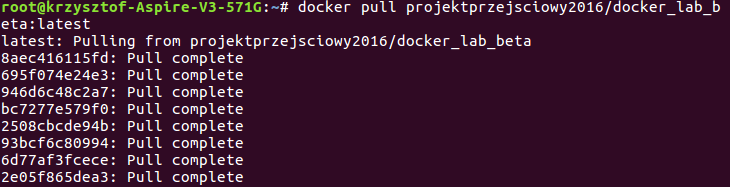
\includegraphics[width=12 cm]{./grafika/pull.png}
 
\end{figure}


Przed uruchomieniem obrazu należy zezwolić wszystkim aplikacjom działającym z poziomu Dockera na uruchamianie się w trybie graficznym:
\begin{verbatim}
 xhost +
\end{verbatim}

Powinien pojawić się następujący komunikat:
$"$access control disabled, clients can connect from any host$"$

Uruchomienie obrazu systemu odbywa się poprzez wpisanie w konsoli polecenia (powoduje stworzenie nowego kontenera, na podstawie wywołanego i otwiera go - wszelkie zmiany będą zapisywane w nowym kontenerze) :

\begin{verbatim}
 docker run -it -e DISPLAY=unix$DISPLAY -v=/tmp/.X11-unix:/tmp/.X11-unix:rw \
 projektprzejsciowy2016/docker_lab_beta:latest

\end{verbatim}

W przypadku gdy potrzebujemy współdzielić pewne katalogi lokalne z Dockerem należy  w poleceniu uruchamiającym obraz systemu $"$docker run$"$ skorzystać z opcji -v:
\begin{verbatim}
docker run -it -e DISPLAY=unix$DISPLAY -v=/tmp/.X11-unix:/tmp/.X11-unix:rw \
-v[scieżka_do_katalogu_lokalnego]:[scieżka_gdzie_ma_być_montowany_w_obrazie] \
projektprzejsciowy2016/docker_lab_beta:latest

\end{verbatim}


System ROS wraz z symulatorem - Gazebo, uruchamiany jest poleceniem wykonywanym już z poziomu obrazu Dockera:
\begin{verbatim}
roslaunch projekt_przejsciowy l15.launch &
\end{verbatim} 

Po chwili powinien uruchomić się symulator Gazebo:

\begin{figure}[hbt]
  \setlength{\unitlength}{1.0cm}
  \centering 
  
    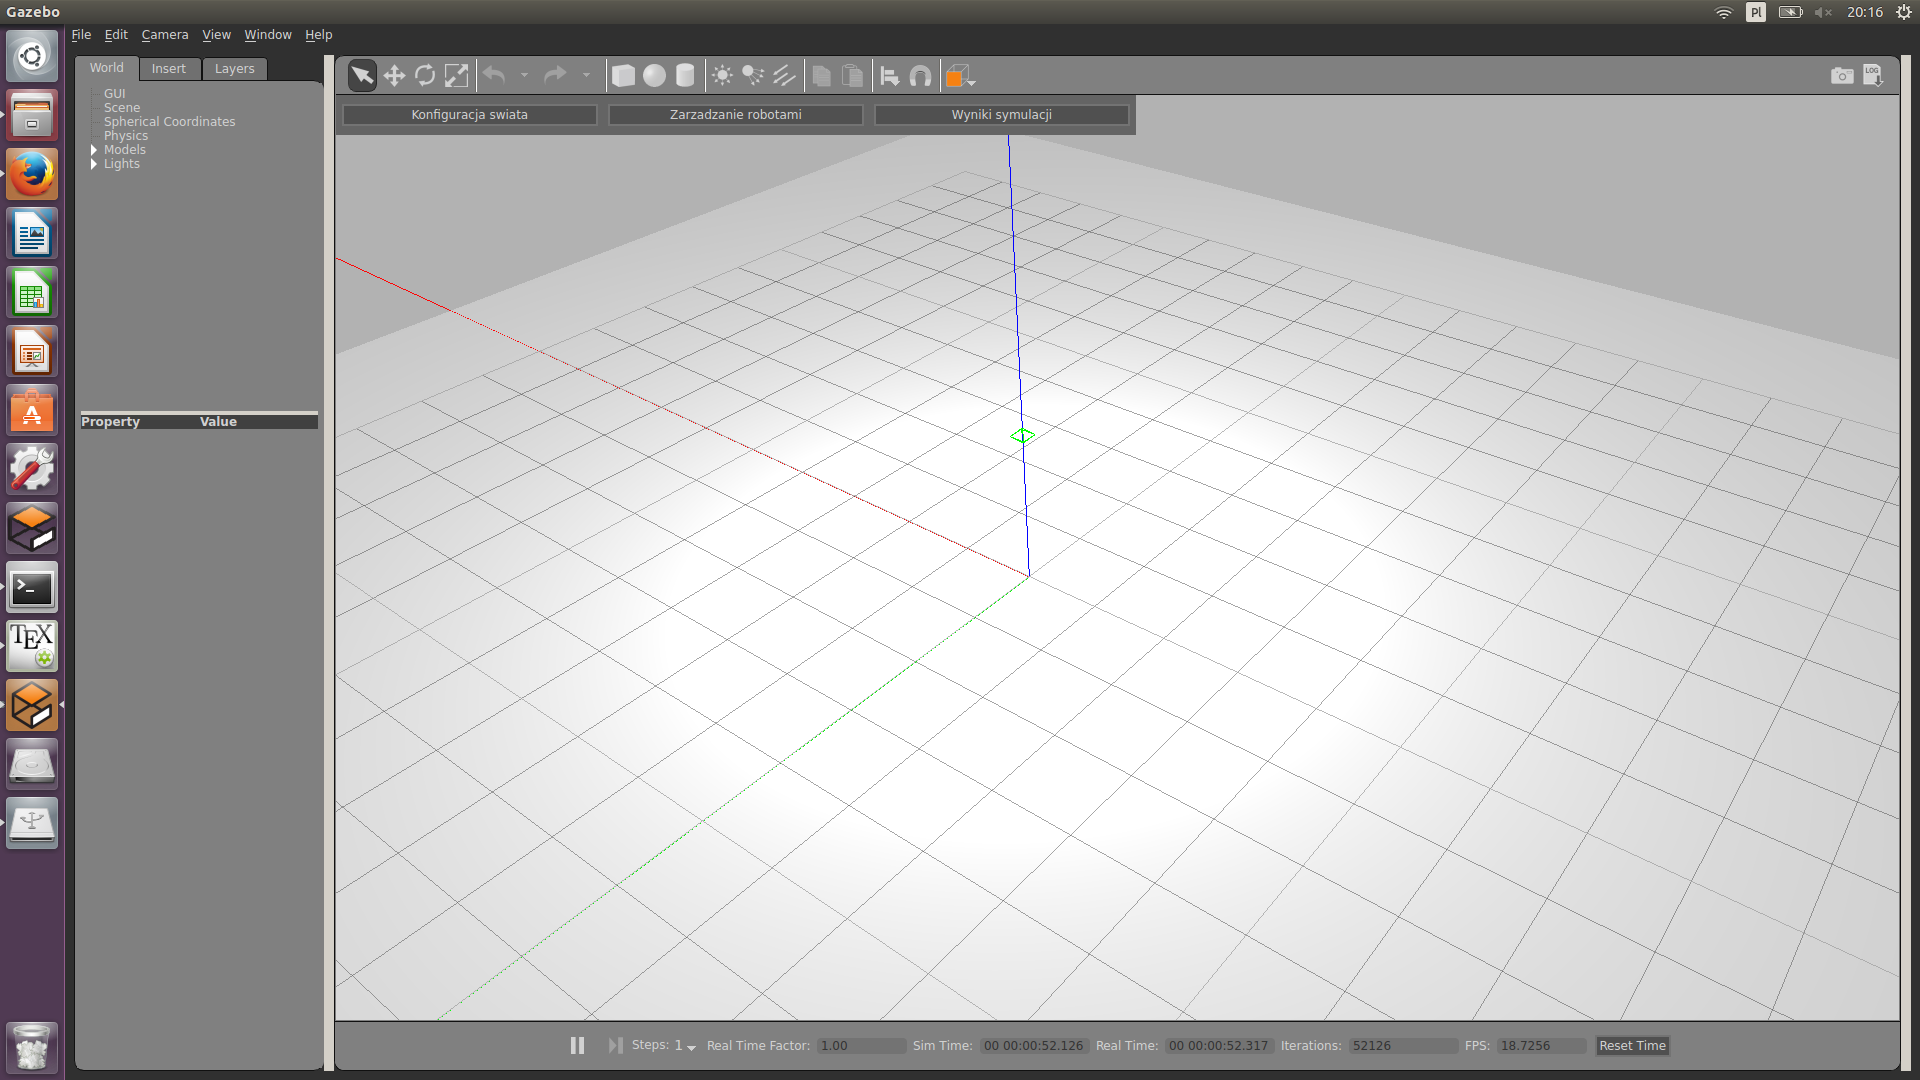
\includegraphics[width=12 cm]{./grafika/EkranGlowny.png}

\end{figure}
 Aby przetestować czy wszystko działa poprawnie należy dodać na scenę robota jak w puncie 3.2.


Jeśli potrzebujemy uruchomić drugą konsolę działającą na tym samym kontenerze to należy uruchomić drugą konsolę (można to wykonać skrótem klawiszowym $"$shitf$"$+$"$ctrl$"$+$"$t$"$, a następnie sprawdzamy nazwę kontenera, który mamy już uruchomiony:

 \begin{verbatim}
docker ps -a
\end{verbatim}


Powyższe polecenia wyświetla listę wszystkich dostępnych lokalnie kontenerów, w której można sprawdzić nazwy poszczególnych kontenerów:


\begin{figure}[hbt]
  \setlength{\unitlength}{1.0cm}
  \centering 
  
    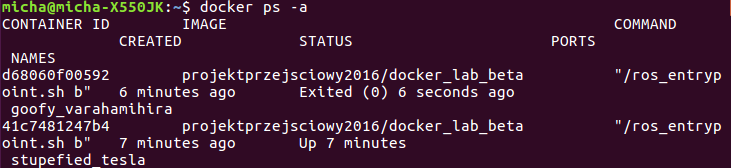
\includegraphics[width=12 cm]{./grafika/ps-a.png}

\end{figure}

Na przedstawionej na rysunku liście przykładowe nazwy to goofy\_varahamihira oraz stupefied\_tesla. Podpięcie się konsolą pod otwarty już kontener opiera się o polecenie:


 \begin{verbatim}
docker exec -it Nazwa_Kontenera bash
\end{verbatim}


Uruchamiając kontener po raz kolejny mamy możliwość zachowania historii wykorzystywanych poleceń. Przy uruchamianiu kontenera odwołujemy się do ostatniego otwieranego dockera:
\begin{verbatim}
docker start -i $(docker ps -q -l)
\end{verbatim}



\section{Obsługa systemu}
\subsection{Dodawanie modelu sali}
Na obrazie systemu, w chwili obecnej, znajdują się trzy przykładowe modele świata:
\begin{itemize}
\item model sali L1.5 w budynku C-16
\item dwa dodatkowe modele składające się z ułożonych w pewien sposób mebli 
\end{itemize}

Dodanie jednego z tych światów możliwe jest z poziomu okna "Konfiguracja Świata". Dostep do wspomnianego okna jest z poziomu widoku głównego Gazebo pod przyciskiem umieszczonym z lewej strony listwy na górze ekranu.
\begin{figure}[hbt]
  \setlength{\unitlength}{1.0cm}
  \centering 
  
    \includegraphics[width=12 cm]{./grafika/KOnfiguracjaSwiata.png}

\end{figure}
W oknie tym, po lewej stronie, znajduje się lista dostępnych światów oraz dwa przyciski "Wczytaj" i "Wyczyść". Wybraną salę można dodać wybierając ją z lisy i klikając pierwszy przycisk. Jeśli wczytamy inną salę w momencie, gdy jakaś jest już wczytana, scena zostanie automatycznie wyczyszczona i wczytany aktualnie wybrany świat. Przycisk "Wyczyść$"$ służy do usunięcia wszystkich obiektów ze sceny z wyjątkiem robotów.

 \subsection{Dodawanie modeli robotów}
Z okna konfiguracji świata można również dodawać na scenę roboty (jak narazie dostępne są trzy roboty Pioneer). Służą do tego listy na środku oraz z prawej strony okienka. Lista środkowa zawiera roboty, które są dostępne do dodania, a prawa te, które są już dodane. Aby dodać robota, należy wybrać go z listy środkowej i kliknąć przycisk " Dodaj". Roboty dodane pojawią się na scenie w momencie kliknięcia przycisku $"$Zatwierdź$"$.  W tym samym momencie pojawiają się w systemie ROS topiki związane z dodawanymi robotami. Listę topików można zobaczyć wpisując w terminalu:
\begin{verbatim}
rostopic list
\end{verbatim}
Przycisk $"$Schowaj" umieszcza wybranego robota poza salą w tak zwanym schowku.

Aby przetestować czy Gazebo dobrze współpracuje z systemem ROS należy dodać robota a następnie w konsoli wydać polecenie publikujące w topicu ROSa odpowiadającym za prędkość dodanego robota:
\begin{verbatim}
rostopic  pub /pionner_1/RosAria/cmd_vel geometry_msgs/Twist \
-- '[1.0, 0.0, 0.0]' '[0.0, 0.0, -0.5]
\end{verbatim}

W efekcie robot powinien zacząć poruszać się po okręgu.

\begin{figure}[hbt]
  \setlength{\unitlength}{1.0cm}
  \centering 
  
    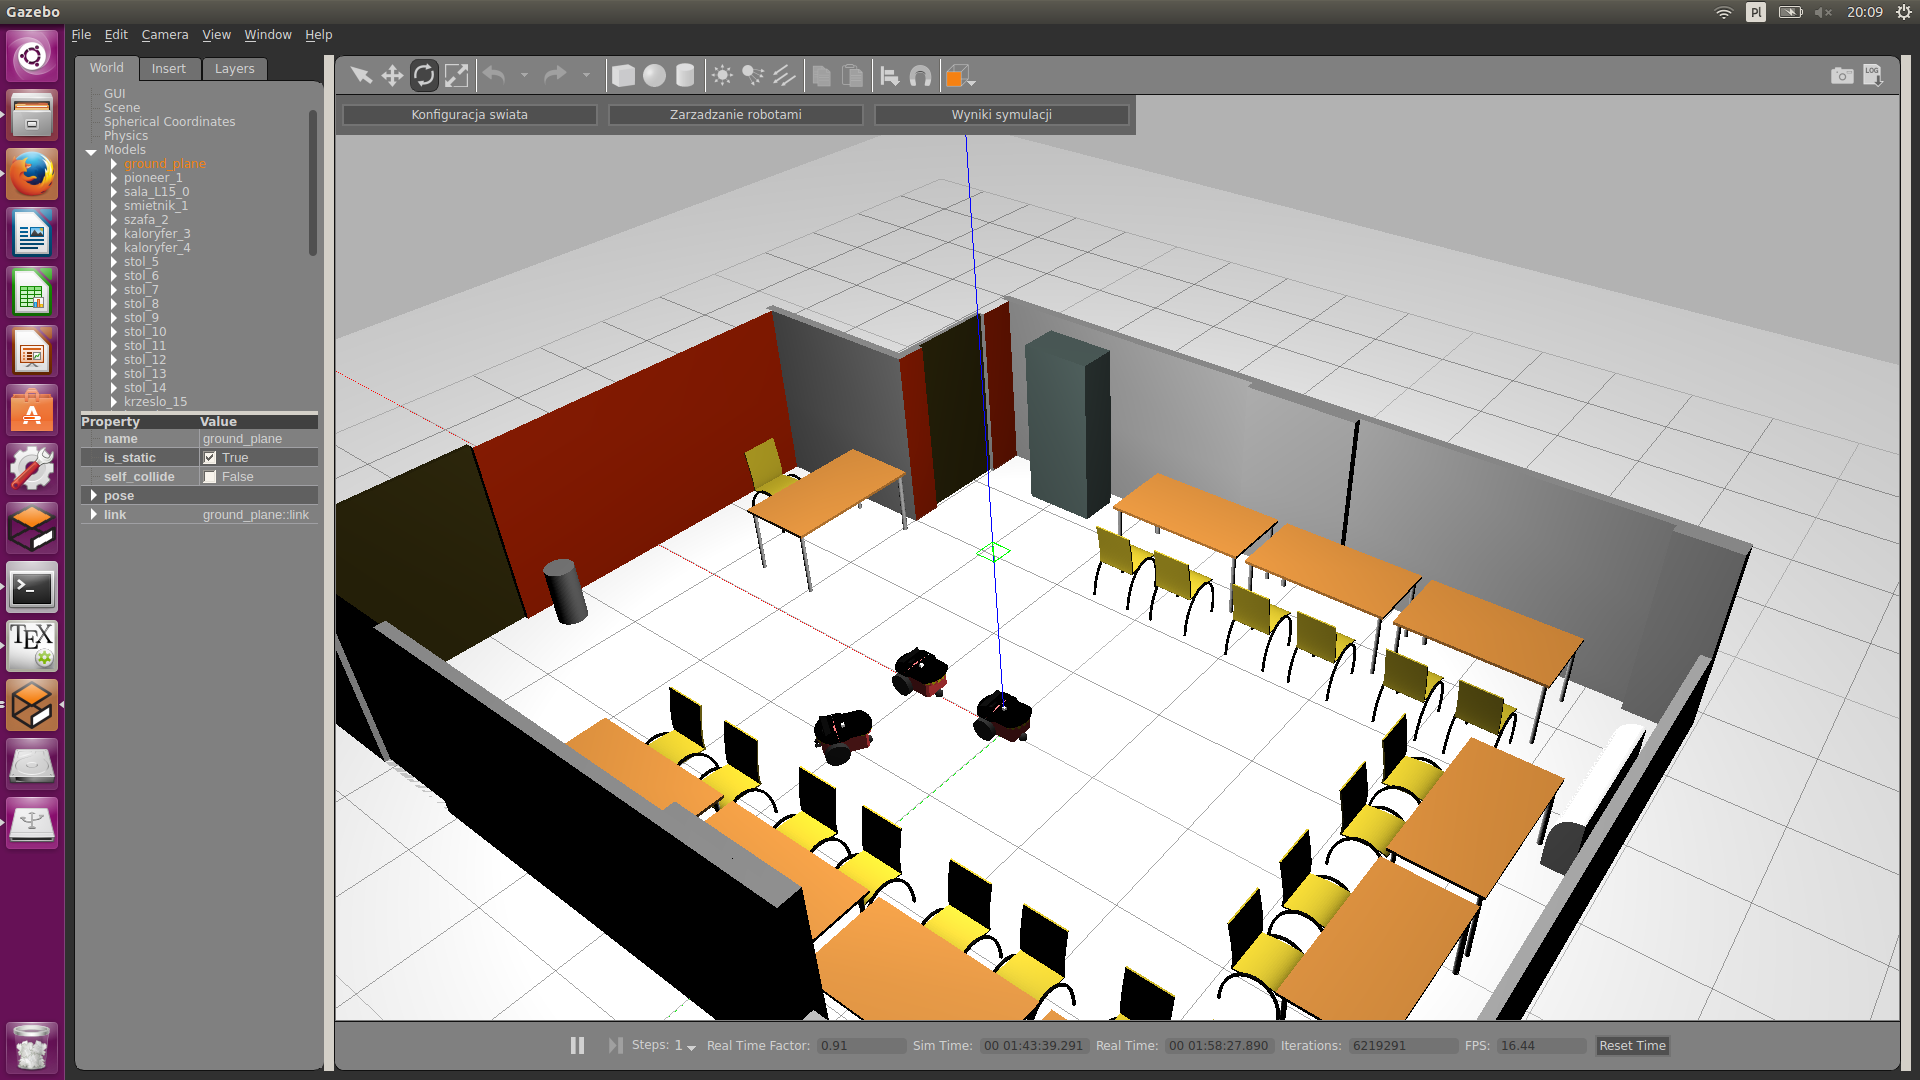
\includegraphics[width=12 cm]{./grafika/EkranGlownyZSalaIRobotami.png}

\end{figure}

 \subsection{Resetowanie robotów i ustawianie ich w zadanych miejscach}

Do resetowania i ustawiania w zadanej pozycji robotów służy okno $"$Zarządzanie robotami". Okno podzielone jest na zakładki - każda z nich dotyczy osobnego robota. Umieszczony w każdej zakładce przycisk $"$Reset$"$ ustawia odpowiedniego robota w punkcie (0,0) sali z orientacją równą 0. Pola tekstowe służą do zadawania pozycji (X,Y) i orientacji robota. Wartości z tych pól są wykorzystywane przy używaniu przycisku "Ustaw". W trakcie kliknięcia wartości te są sprawdzane i ich ewentualna niepoprawność jest sygnalizowana czerwonym podświetleniem pola. Dopiero po sprawdzeniu robot przemieszczany jest na ustaloną pozycję.
\begin{figure}[hbt]
  \setlength{\unitlength}{1.0cm}
  \centering 
  
    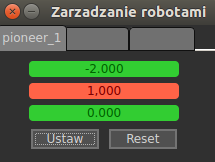
\includegraphics[width=6 cm]{./grafika/OknoZarzadzaniaRobotami.png}

\end{figure}


\subsection{Wyświetlanie i zapisywanie wyników}
Do wizualizacji i zapisu danych z eksperymentu przygotowane zostało okno $"$Wyniki symulacji$"$. Okno podzielone jest na zakładki, w których można otrzymać podgląd trajektorii wszystkich robotów oraz przebiegi położenia X, Y i orientacji. W pierwszej zakładce są trasy przebyte przez wszystkie roboty a każda kolejna zakładka odnosi się do konkretnego robota prezentując jego położenie i orientację. Przycisk $"$Reset danych$"$ pozwala wyczyścić wykresy i zacząć zbierać je od nowa.  Okno daje możliwość zapisania przebiegów do plików, które znajdują się potem w folderze /root/.  Ważne jest też aby przed rozpoczęciem zbierania danych do konkretnego wykresu za pomocą przycisku z dolnego paska Gazebo $"$PLAY/PAUSE$"$ zatrzymać czas symulacyjny następnie przyciskiem $"$Reset Time$"$ aby wykres był czytelny.
\begin{figure}[hbt]
  \setlength{\unitlength}{1.0cm}
  \centering 
  
    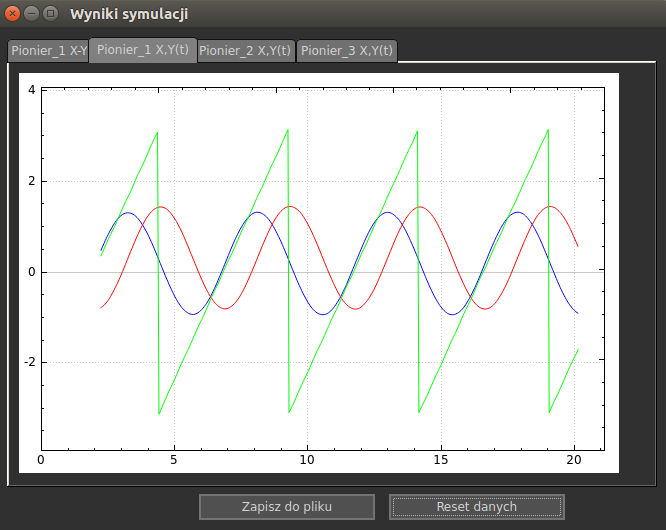
\includegraphics[width=6 cm]{./grafika/Wykres.png}

\end{figure}

\subsection{Wyświetlanie odczytów z czujników}
Aby uzyskać dostęp do pomiarów z czujników należy z paska narzędzi Gazebo wybrać zakładkę $Window$ $>>$ $Topic$ $Visualization$. Uruchomi się okno:
 \begin{figure}[hbt]
  \setlength{\unitlength}{1.0cm}
  \centering 
  
    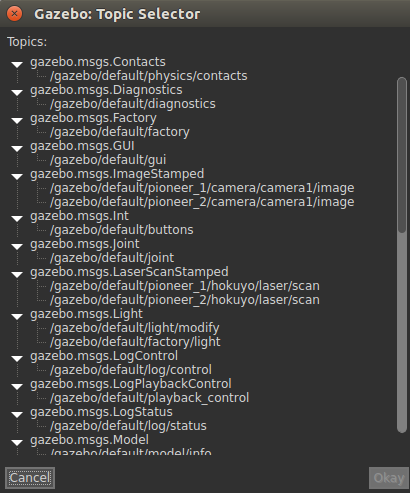
\includegraphics[width=6 cm]{./grafika/WizualizacjaLista.png}

\end{figure}

Następnie wybieramy topic czujnika, z którego chcemy wyświetlać dane. Dla skanera laserowego wykres wygląda następująco:

 \begin{figure}[hbt]
  \setlength{\unitlength}{1.0cm}
  \centering 
  
    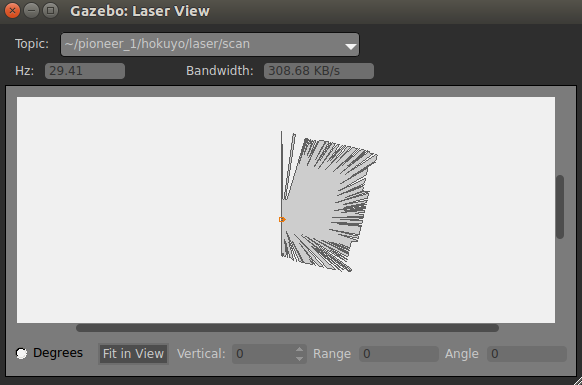
\includegraphics[width=8 cm]{./grafika/Skaner.png}

\end{figure}
\newpage
\subsection{Dodawanie i edycja modeli przeszkód na scenie}
Aby dodać przeszkodę na scenę należy z lewej strony ekranu wejść w zakładkę "Insert", wybrać kliknięciem model i kliknąć na miejsce na scenie, w którym chcemy postawić przeszkodę. Proste modele przeszkód dostępne są z paska narzędzi Gazabo. 
Aby zmienić statyczność przeszkody należy kliknąć na nią prawym przyciskiem myszy (PPM) a następnie z rozwiniętego menu wybrać opcję $"$Edit Model". Gazebo przejdzie do trybu edycji modelu. Wybieramy zakładkę "Model" i zaznaczamy lub odznaczamy opcję $"$Static":

\begin{figure}[hbt]
  \setlength{\unitlength}{1.0cm}
  \centering 
  
    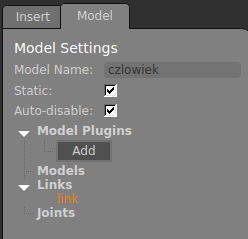
\includegraphics[width=6 cm]{./grafika/Edit.png}

\end{figure}



\end{document}
 

\chapter{Instrukcja dla dewelopera}
\section{Wst�p}

W niniejszej instrukcji znajduje si� opis wst�pnych czynno�ci wymaganych do dalszego rozwoju symulatora. Prezentuje konfiguracj� narz�dzi, �rodowiska oraz obrazu a tak�e automatyzacj� procesu budowy obrazu dla wersji deweloperskiej oraz testowej/finalnej przy pomocy pliku Dockerfile.\\
Instrukcja opisuje stan na stycze� 2017 roku, przez co informacje w niej zawarte mog� by� nieaktualne. Dotyczy to system�w operacyjnych wspieraj�cych Dockera, dost�pnej wersji ROS'a oraz Gazebo, a tak�e API, z kt�rego korzystano.  
%
\section{System}
\label{sec:system}
Wymagany jest system Linux w architekturze 64 bitowej. Wybrane wspierane dystrybucje \textbf{Ubuntu}:
\begin{itemize}
	\item Yakkety 16.10
	\item Xenial 16.04 (LTS)
	\item Trusty 14.04 (LTS)
\end{itemize}
\textbf{Debian}:
\begin{itemize}
	\item Jessie 8.0 (LTS)
	\item Wheezy 7.7 (LTS)
\end{itemize}
Pe�na lista wspieranych dystrybucji dost�pna jest pod adresem \url{https://docs.docker.com/engine/installation/linux/}.
Praca z Dockerem mo�liwa jest r�wnie� na systemie Windows, ale niniejsza instrukcja nie zawiera opisu dla tego systemu, gdy� nie uda�o si� skonfigurowa� �rodowiska do pracy z Dockerem w trybie graficznym.

\section{Docker}
Oprogramowanie nale�y zainstalowa� zgodnie z instrukcj� przygotowan� dla wybranego systemu operacyjnego umieszczon� na stronie dostawcy (link z podpunktu \ref{sec:system}).

\section{Obraz}
Symulator mo�na rozbudowywa�, dzi�ki przygotowanemu obrazowi, dost�pnego na~platformie \textbf{DockerHub} pod adresem \url{https://hub.docker.com/r/projektprzejsciowy2016/docker_lab/}. Sk�ada si� z systemu operacyjnego \textbf{Ubuntu Xenial 16.04 LTS}, systemu \textbf{ROS Kinetic} oraz \textbf{Gazebo 7.5} oraz pozosta�ych narz�dzi do komunikacji ROS-Gazebo. Je�eli zaprezentowana konfiguracja jest akceptowalna przez dewelopera, nale�y pobra� obraz. W przeciwnym wypadku nale�y zapozna� si� z rozdzialem \ref{sec:dockerfile}, w kt�rym przedstawiono, jak przy pomocy pliku Dockerfile mo�na wygenerowa� nowy obraz.

\section{Dockerfile}
\label{sec:dockerfile}
\bibliographystyle{plabbrv}
\nocite{*}
\bibliography{raport}

\end{document}
